% !TEX encoding = UTF-8 Unicode
\documentclass[12pt,english]{article}
\usepackage[utf8]{inputenc}
\usepackage{graphicx}
\usepackage{anysize}
\usepackage{hyperref}
\usepackage{float}
\usepackage{caption}
\marginsize{2cm}{2cm}{1cm}{3cm}
\parskip 2ex
\parindent 0cm
\renewcommand{\contentsname}{Contenidos}
\renewcommand\figurename{Figura}
\title{Práctica 3\\ Entrada y salida de datos utilizando el texto}
\author{Lluis Ulzurrun De Asanza Sàez\\Victor Grau Moreso \\Mark Antony Holland}
\date{}

\begin{document}

    \maketitle

    \tableofcontents

    \newpage
    
    \section{Introducción}

    Comprobado que tenemos en local tanto la documentación como los ejemplos de DEVKITPRO.

    \section{Gestión de los controles}

    Hemos realizado un program que imprima por pantalla el estado de los 13 botones mediante el enum \texttt{KEYPAD\_BITS} y la función \texttt{keysHeld()}. El color del texto cambia dependiendo de si está pulsado o no ese boton.
    
    \begin{figure}[H] 
    \centering
    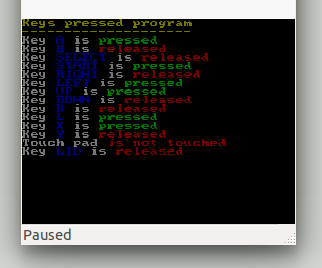
\includegraphics[scale=0.5]{images/keysHeld}
    \caption{Captura del programa keysHeld.}
    \end{figure}

    \newpage

    \section{Uso avanzado del texto en pantalla}

    \subsection{custom\_font}

    En este ejemplo han creado un fichero \textbf{.bmp} que contiene por filas en una columna 95 caracteres. El programa utiliza el fichero \texttt{font.h} creado por grit y este \textbf{.bmp} para definir un variable de tipo ConsoleFont y luego lo utiliza con un \texttt{console} definido al principio del programa. Al final del programa con un simple \texttt{printf} nos muestra en el emulador la fuente custom.

    \begin{figure}[H] 
    \centering
    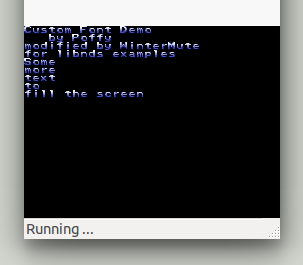
\includegraphics[scale=0.5]{images/custom_font}
    \caption{Captura del programa custom\_font.}
    \end{figure}

    \subsection{print\_both\_screens}

    \subsection{rotation}

    \subsection{rotscale\_text}

    \subsection{console\_windows}
      
    
    
\end{document}